% 2008 年四川延考区卷理科第 12 题：正方体的展开图，B、C、D 为原正方体顶点，A 为一条棱的中点。
% 来源 PDF：gaokaomath-src/普通高考/2008/2008延考区理.pdf
% SHA-256：fd43150eef7b5ad202debed91a533c5cc7764d63e284afbc45b5dedbff457f61
% 原页：2008延考区理.pdf 第 2 页（A4 单栏），题面第 12 题的配图。
% 绘制依据：按原页画六个单位正方形（横排四个，第一个上方一个、第三个下方一个），
%   标出顶点 B(1,1)、C(3,0)、D(4,1) 与棱中点 A(0,1.5)，并画出 AB、CD 两条线段。
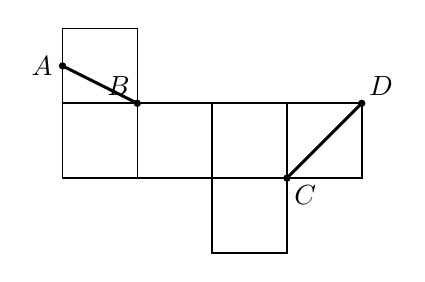
\begin{tikzpicture}[scale=0.95, semithick, every node/.style={inner sep=1.4pt}]
  % 横排四个正方形
  \draw (0,0) rectangle (4,1);
  \draw (1,0) -- (1,1);
  \draw (2,0) -- (2,1);
  \draw (3,0) -- (3,1);
  % 第一个正方形上方一个
  \draw (0,1) rectangle (1,2);
  % 第三个正方形下方一个
  \draw (2,-1) rectangle (3,0);

  % 题干给出的两条线段
  \draw[line width=1.1pt] (0,1.5) -- (1,1);
  \draw[line width=1.1pt] (3,0) -- (4,1);

  \fill (0,1.5) circle (1.4pt);
  \fill (1,1) circle (1.4pt);
  \fill (3,0) circle (1.4pt);
  \fill (4,1) circle (1.4pt);

  \node[left=2pt] at (0,1.5) {$A$};
  \node[above left=1pt] at (1,1) {$B$};
  \node[below right=1pt] at (3,0) {$C$};
  \node[above right=1pt] at (4,1) {$D$};
\end{tikzpicture}
